\section{Anforderungsanalyse}

\subsection{Systembeschreibung}

    Die zu entwickelnde Anwendung verfolgt einen datengetriebenen Ansatz. Daten aus dem Argo-Programm werden erhoben und eine Auswahl davon in ein Datenformat überführt. Zur Darstellung wird eine Webapplikation verwendet. Über diese werden   über Postionsmarker auf einer Weltkarte, die letzten Positionen der Messstationen angezeigt.  Über einen Klick auf die Repräsentation einer Messboje werden weitere Daten der Messstation präsentiert.
    
    

% BEGIN ermittlung  Anforderungen 
    \subsection{Ermittlung der Anforderungen}
    
    Ausgehend von einem ersten Prototypen wurden Use-Cases entwickelt(Siehe Abbildung \ref{fig:use_case}). Dabei wurden zwei Klassen von Akteuren herausgearbeitet. Darunter finden sich die Benutzenden, also die eigentlichen Anwender der Applikation. Diese erwarten einen reibungslosen Betrieb der Applikation und die Darstellung der Messstationen in der gegebenen Form. Zum anderen existiert die Klasse der Administrierenden. Diese benötigen Werkzeuge um die Daten zu restrukturieren und in die Datenhaltung einzuspielen. Beide Klassen haben verschiedene Sichten auf die Datenhaltung. Daraus entsteht ein Spannungsverhältnis, welches minimiert werden muss.
    
    \begin{figure}[h!]
        \centering
        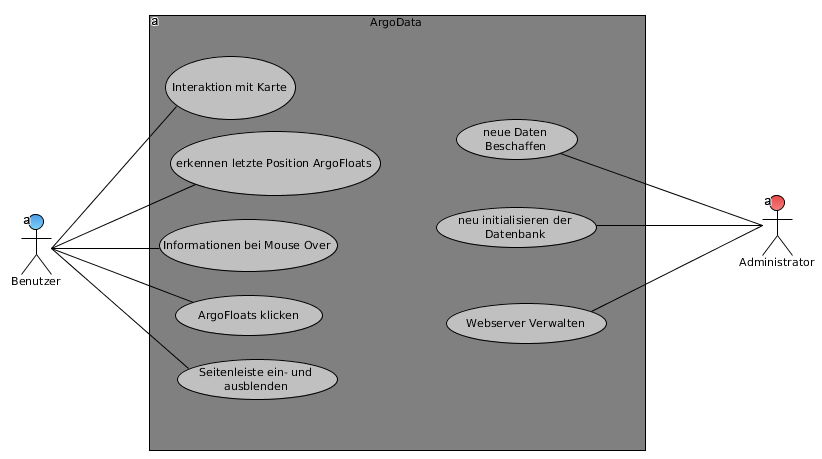
\includegraphics[width=0.8\textwidth]{pix/use-case.png}
        \caption{Use case Diagramm der Anforderungen}
        \label{fig:use_case}
    \end{figure}
    
    Anhand dieses Modelles  wurden Anforderungen ausgearbeitet. Diese wurden in Form eines gerichteten Graphen aufbereitet (Siehe Abbildung: \ref{fig:graph_anforderungen}). Dabei werden die Anforderungen und deren Nachbedingungen über Knoten des Graphen repräsentiert. Finden sich in einer Anforderung Vorbedingungen zu den Nachbedingungen einer anderen Anforderung, so wird diese Abhängigkeit über eine Kante dargestellt. Diese Darstellung half dabei, Definitionslücken in den Beziehungen  der Anforderungskette besser verstehen zu können und formale Lücken schließen zu können.
      
    \begin{figure}[h!]
    \centering
    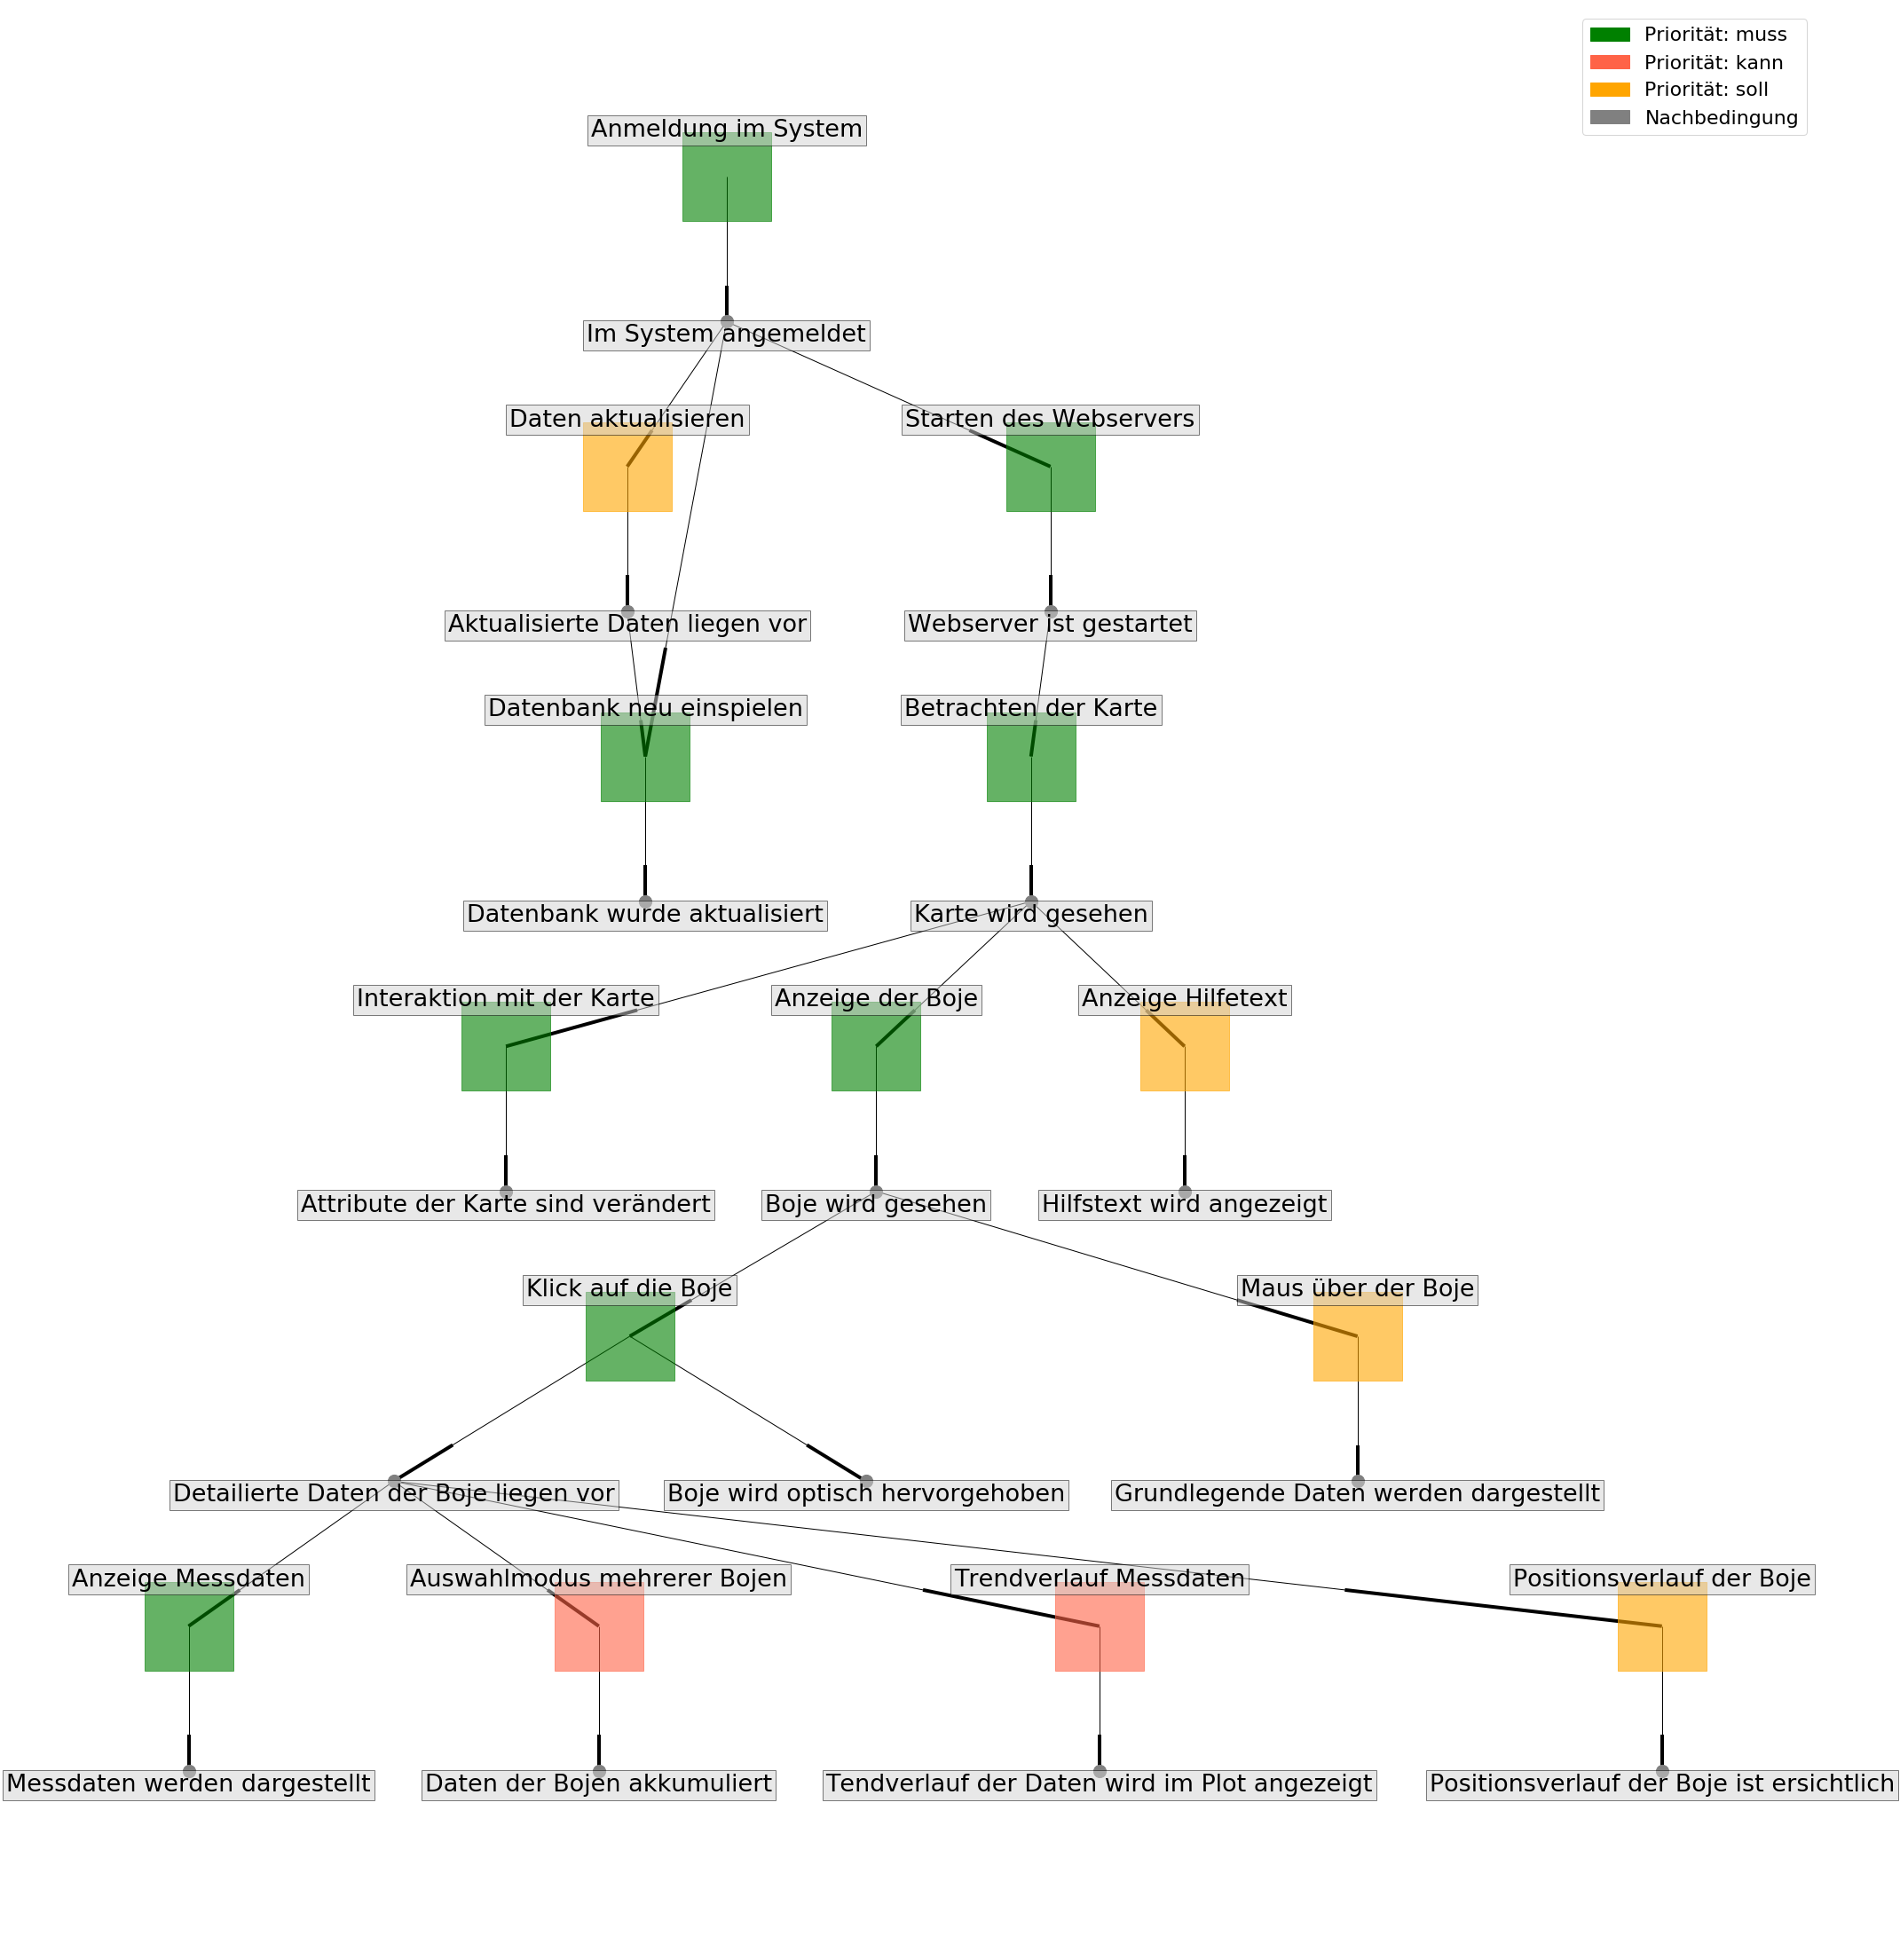
\includegraphics[width=\textwidth]{pix/graph_anforderungen.png}
    % graph_anforderungen.png: 1208x850 px, 72dpi, 42.63x29.99 cm, bb=0 0 1208 850
    \caption{Anforderungen und ihre Abhängigkeiten als gerichteter Graph}
    \label{fig:graph_anforderungen}
    \end{figure}
    
% END 
     
% BEGIN Beschreibung  funktionale Anforderungen
    \subsection{Funktionale Anforderungen}
    
    \subsubsection{Anwendende Perspektive}
    
    In der Anwendung wird die Darstellung einer Webapplikation erwartet. Angesteuert durch die zugehörige URL 
    sollen über eine Kartenapplikation die Grenzen der Ozeane und der umliegenden Kontinente erkennbar werden.  Eine genauere Darstellung von Landmarken wie Straßen, Städte oder Gebirge ist für den Aussagewert der Applikation nicht erforderlich. Die Kartendarstellung soll über Interaktionsmöglichkeiten, wie dem Einstellen der Zoomstufe, sowie des ausgewählten Kartenbereichs, verfügen. Über den Kartendienst sind die letzte Position jeder Messboje aus dem Datensatz ersichtlich. Um Streuung und Verdichtung an spezifischen Orten sehen zu können, werden alle Bojen des angezeigten Kartenausschnittes dargestellt. Es erfolgt keine Zusammenfassung oder Ausblendung.
    Wird die Maus über die visuelle Repräsentation einer Messboje geführt, so sollen grundlegende Daten der Messstationen dargestellt werden, gleichzeitig wird diese Station optisch hervorgehoben.
    Ein Mausklick auf die schematische Darstellung soll hier gemessene, spezifische Daten anzeigen. Dazu werden in einem separierten Darstellungsfeld der Verlauf der Messdaten, sowie weiterer sinnvoller Werte angezeigt. Zusätzlich soll der zurückgelegte Weg der Messtation ersichtlich sein.  Eine Trendanalyse der Daten könnte hier ein Maß für die Richtung der Messwerte ermöglichen. Könnten mehrere Messstationen gleichzeitig ausgewählt werden, so wäre es sinnvoll die akkumulierten Werte darzustellen.
    
    \subsubsection{Administrative Perspektive}
    
    Es notwendig, dass die Datensätze des Argo Programms ausgelesen und in ein für die Datenbank aufbereitetes Format überführt werden. Neue Daten müssen hierfür aus den Quellen des Argo Programms heruntergeladen werden. Um die Inhalte zu erstellen, werden statt einer journalistischen eine administrative Tätigkeiten erwartet. Durch den Datengetriebenen Ansatz der Applikation müssen für das Erstellen der Inhalte keine Webmasken wie Texteingabefelder zur Verfügung gestellt werden. Vielmehr ist es hier sinnvoll, die hier benötigten Werkzeuge als Skripte zur Verfügung zu stellen, um die administrativen Aufgaben über die Kommandozeile ausführen zu können. Dies würde eine Abbildung der Prozesse bis hin zu einer Vollautomatisierung erlauben und eine örtliche Trennung von Datenaggregation und -darstellung vereinfachen.
    Für die administrativen Tätigkeiten werden Werkzeuge benötigt, um neue Daten  in die Datenbank überführen können.  
% END 
    

% BEGIN Beschreibung  nicht-funktionale Anforderungen


\subsection{Nicht-Funktionale Anforderungen}
    
    \subsubsection{Anwendende Perspektive}
        Für die Benutzenden sind Usability und Benutzbarkeit der wichtigste Aspekt. Die Bedienungsmuster müssen klar ersichtlich und intuitiv erfahrbar sein. Die Darstellung der Applikation soll einfach und schlicht gehalten werden und dem gewohnten Erscheinen modernen Web Applikationen entsprechen. 
        Es soll Wert auf die wichtigsten Aspekte des Datenschutzes Wert gelegt werden. Insbesondere im Hinblick auf Datensparsamkeit sind das Einbinden von Trackern, Loginfunktionen und das Speichern von Logfiles zu bewerten.
        Sicherheitsaspekten ist aus der Anwendersicht nur eine normale Rolle zugewiesen werden. Dabei sollen die heute normalen Sicherheitsvorkehrungen, wie zum Beispiel Transportverschlüsselung und Schutz gegen SQL-Injections erfolgen.
        
    \subsubsection{Administrative Perspektive}
        Für die Aggregation der Daten ist die Sicherheit ein zentraler Aspekt. Dies umfasst sowie Aspekte von Authentifizierung und Autorisierung der Rolle der Datenaggregation als auch eine Sicherheit um die Integrität der Heruntergeladenen Daten.
        
    
% END 

% BEGIN Auswahl der Daten
\subsection{Benötigte Daten}

Um die Darstellung zu vereinfachen und die Kommunikation mit der Datenbank zu beschleunigen, ist im ersten Schritt eine Auswahl aus den Daten der Argo-Bojen vorzunehmen. Hierbei soll darauf geachtet werden, nur diejenigen Daten zu verwenden, welche für die Erbringung des Dienstes notwendig sind.

Aus diesem Grund findet sich im Folgenden eine Auswahl aus dem Datenkatalog \footnote{Siehe Quelle \cite{ArgoUserManual} S. 19 ff.} von Argo mit der jeweiligen Begründung:

\begin{center}
\begin{table}
  \label{table:Datenauswahl}
  \begin{tabular}{ | l | p{7cm}| c |}
    \hline
    \textbf{Datenfeld} & \textbf{Beschreibung} & \textbf{Datentyp} \\\hline
   
    PLATFORM\_NUMBER 
        &  Eindeutige Identifikationsnummer einer einer Messstation
        & <STRING8>
        \\\hline 
    
    CYCLE\_NUMBER 
        &  Fortlaufende und innerhalb einer Messboje eindeutige Identifikationsnummer eines Messprofils
        & <int32>
        \\\hline
    
    JULD
        & In Julian Date codierter Zeitpunkt der Übertragung (Begin oder ende?) einer Messung
        & <float64>
       \\\hline
        
    N\_PARAM
        & Anzahl der Messsensoren. 
        & <STRING16>
        \\\hline
        
    LATITUDE \& LONGITUDE
        & Die Positionsdaten einer Messung zum Zeitpunkt der Übetragung der Werte.
        & <float64>
        \\\hline
        
    PRES
        & Messvektor des Wasserdrucks
        & <float32>
        \\\hline
        
    TEMP
        & Messvektor der Wassertemperaturen 
        & <float32>
          \\\hline
        
    PSAL
        & Messvektoren des Salzgehaltes
        & <float32>
         \\\hline
    \end{tabular}
      \caption{Beschreibung der ausgewählten Daten}
\end{table}
\end{center}

Das Feld PLATFORM\_NUMBER wird benötigt um Messprofile eindeutig der Plattform zuordnen zu können. Während die CYCLE\_NUMBER eine Messung innerhalb ihrer Plattform eindeutig zuordenbar macht. Das Datum der Messdatenübertragung kann aus dem Feld JULD ermittelt werden, dieses erlaubt es, die Messreihe in ihren zeitlichen Kontext zu sehen. Die Anzahl der Sensoren lässt sich aus dem Feld N\_PARAM herleiten. Dies wird benötigt, da einige Messstationen nicht alle Sensoren eingebaut haben. Über die Geokoordinaten wird die lokale Zuordnung der Datenübertragung erreicht. Dies wird benötigt um in der Kartendarstellung der Messung einen Ort zuzuweisen.
Aus den Messwerten werden die Felder PRES, TEMP und PSAL ausgewählt. Neue Modelle von Argo Floats besitzen noch das Feld COND über den sich die Leitfähigkeit des umliegenden Wassers herleiten lässt. Dieser ist aber noch nicht bei vielen Messstationen implementiert und wird deswegen hier nicht verwendet.


 

%TODO Der kleine Satz möchte aus den Untiefen der Schachtelsätze abgeholt und verbessert werden
\paragraph{Vereinfachung der Messdaten}
Die verwendeten Messwerte PRES, TEMP und PSAL eines Messprofils liegen in Vektorieller Form vor. Für die Darstellung über einen univariaten Graphen wird nur ein skalarer Wert pro Messprofil benötigt. Die Daten sollen zusammengefasst werden, bevor diese in die Datenstruktur überführt werden um die Größe der Daten zu verringern. 
%TODO Implementierung welcher Algorithmus zurzusammenfassung 
 
% END 

% BEGIN technische Anforderungen
\subsection{Technische Anforderungen  }

\subsubsection{Verwendete Programmiersprachen}

Die Darstellung der Webapplikation wird mit HTML und Javascript umgesetzt werden. Diese Sprachen gelten in der Entwicklung von Webseiten als Standard und werden von den gängigen Browsern unterstützt.

Die weiteren teile der Applikation soll mit einer Sprache entwickelt werden, die alle benötigten Teilbereiche umsetzen kann.

Das \textbf{Öffnen der netCDF} Dateien und die numerische Berechnung kann mit C, Java/Scala, R und Python erfolgen. Insbesondere die beiden letzten sind in der Datenverarbeitung und Numerik als etablierte Werkzeuge zu sehen.

Die Darstellung der Seite soll durch ein Webframework unterstützt werden. Hier gibt es in beinahe allen Hochsprachen entsprechende Werkzeuge. Wählt man aus der Problemstellung der numerischen Verarbeitung R und Python heraus, so ist die Auswahl der geläufigen Webframeworks bei Python höher anzusehen. Diese Sprache besitzt eine große Anzahl von Bibliotheken für die Anbindung von Datenbanken, sowie einige etablierte Bibliotheken für die Schaffung von Webapplikationen.  

Python besitzt in Hinsicht auf Laufzeitkosten und einer nicht strikten Typisierung einige Nachteile gegenüber Sprachen wie C und Java. In Hinsicht die auf Auswahl von Programmbibliotheken, sowie der numerischen Berechnung besitzt die Sprache aber Vorteile und wird deswegen hier für die Implementierung genutzt.



\subsubsection{Betriebssystem des Servers}


Für die Laufzeitumgebung der Applikation wird ein GNU/Linux eingesetzt werden. Die Software wird so entwickelt das sie unter den gängigen Distributionen lauffähig sein wird. Für diese Applikation wird sich hier für die Distribution Debian-Stable entschieden. Diese zeichnet sich insbesondere gegenüberweiteren Distribution mit einer ähnlichen Verbreitung wie RHEL und Ubuntu durch ihre nicht kommerzielle Ausrichtung aus. Debian ist sehr verbreitet und stark auf Stabilität ausgelegt. Als Nachteil ist der fehlende kommerzielle Support zu sehen. Diese Arbeit sollte voraussichtlich aber in keine Bereiche vordringen, welche einen kostenpflichtigen Support rechtfertigen würde.

\subsubsection{Webframework}

Für Python gibt es eine große Anzahl an Werkzeugen für die Entwicklung von Webseiten. Hier werden exemplarisch 3 herausgegriffen und für die hier vorliegende Aufgabe bewertet.

\begin{description}
 \item [Django] wird beworben als \texttt{The web framework for perfectionists with dead\-lines}. Es wurde 2005 unter einer BSD Lizenz released und entwicklet, die News-Seite des \textit{Lawrence Journal-World} umzusetzen und zu verwalten. Django ist ein etabliertes und häufig verwendetes Webframework. Es ist dynamisch einsetzbar und für eine große Anzahl von Anwendungen verwendbar. Die Bibliothek ist außerdem durch Module erweiterbar. Die Software folgt dem "`\textit{batteries included}"' Ansatz und liefert in der Grundausstattung bereits alles nötige mit, um eine Webseite inklusive Login und Eingabemasken für journalistische Tätigkeiten auszubauen.
 
 \item [Flask] ist ein sogenanntes Micro-Framework. es verwendet die Toolsammlung \textit{Werkzeug} um Webseiten darstellbar zu machen. Das Farmework folgt dem KISS Ansatz und liefert im Grundumfang nur diejenigen Werkzeuge, die man für die Verwaltung von einfachen Webseiten benötigt. Die Software lässt sich über Module erweitern. Einzelne Teilprojekte von Applikationen lassen sich in sogenannte Blueprints modularisieren. 
 
 \item [Falcon] ist ebenso als Microfarmework zu sehen. Es wurde insbesondere in Hinblick auf Geschwindigkeit entwickelt. Das Framework erlaubt requests asynchron zu verarbeiten und lässt die auf Geschwindigkeit spezialisierte Python-Laufzeitumgebung pypy zu. Falcon ist ein relativ neues Framework und erfährt in letzter zeit zur Schaffung von REST-APIs immer mehr Aufmerksamkeit. Es ist aber auch möglich, mit diesem Framework Webapplikationen mit einer Anzeige über HTML-Elementen zu gestalten. 
\end{description}

In dieser Applikation wird die Schaffung von Journalistischen und redaktionellen Inhalten eine sehr geringe Rolle spielen. Unter diesem Gesichtspunkt ist die Frage der Komplexität der verwendeten Software zu klären. (..) Unter diesem Aspekt erscheint Django nicht als die ideale Wahl.

Flask und Falcon verfogen beide den Ansatz eines Microframeworks. Die Laufzeitgeschwindigkeit des Controllers erscheint an dieser Stelle nicht als limitierender Faktor der Applikation. Zwar wäre es wünschenswert, die Datenbeschaffung der Webapplikation bereits im Backend asynchron zu erledigen, doch überwiegt das breitere Spektrum an Modulen und Dokumentationen für die Webentwicklung von Flask.

Damit erscheint Flask als das geeignetste Werkzeug für diese Aufgabe.


\subsubsection{Datenbank}

Das DBMS soll über Schnittstellen in den Sourcecode des Programmes eingebunden werden. Die datenbank soll einem relationalen schema folgen. Die Verwendung sollte kostenfrei möglich sein und die benötigte Software über die Quellen des betriebssystems verfügbar sein. 

In dieser Applikation wurde sich für die Verwendung von PostgreSQL entschieden. Als Object-Realational-Mapper steht für Python SQLAlchemy zur verfügung.


% END  
